\documentclass{article}


\usepackage{Sweave}

\begin{document}
\subsection*{Introduction}

We generate 3D gaussian data,
We generate 3D Gaussian data,
\begin{Schunk}
\begin{Sinput}
R> set.seed(1)
R> n <- 100
R> x <- rnorm(n); y <- 2*x + rnorm(n)/2
R> U3 <- cbind(x, y, z = -3*x + y + rnorm(n)/4)
\end{Sinput}
\end{Schunk}
look at its structure
\begin{Schunk}
\begin{Sinput}
R> str(U3) # its structure ((comment kept))
\end{Sinput}
\begin{Soutput}
 num [1:100, 1:3] -0.626 0.184 -0.836 1.595 0.33 ...
 - attr(*, "dimnames")=List of 2
  ..$ : NULL
  ..$ : chr [1:3] "x" "y" "z"
\end{Soutput}
\end{Schunk}
and load package \texttt{lattice}
\begin{Schunk}
\begin{Sinput}
R> if(!require("lattice")) q("no")
\end{Sinput}
\end{Schunk}
to visualize it by a simple scatter plot matrix
\begin{figure}[h!]
\centering
\begin{Schunk}
\begin{Sinput}
R> splom(U3, xlab ="", cex = 0.4)
\end{Sinput}
\end{Schunk}
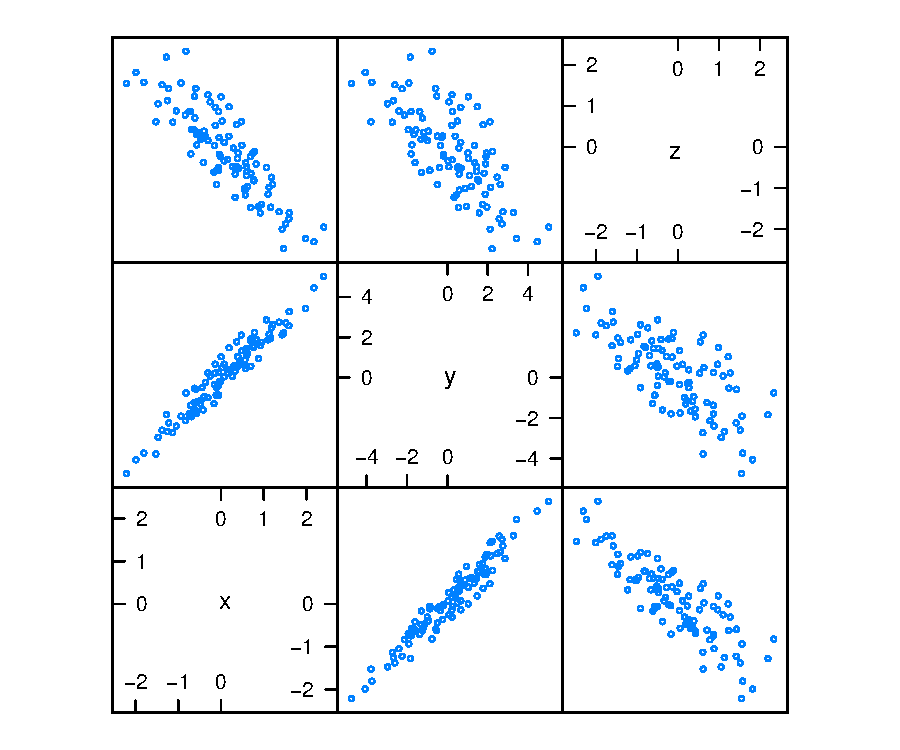
\includegraphics{swv-keepSrc-1-splom}
\caption{100 vectors of random variates ... ...}
\label{fig:AC_Joe}
\end{figure}

\subsection*{Session Information}

\begin{Schunk}
\begin{Sinput}
R> toLatex(sessionInfo())
\end{Sinput}
\begin{itemize}\raggedright
  \item R version 3.6.0 (2019-04-26), \verb|x86_64-apple-darwin15.6.0|
  \item Locale: \verb|en_US.UTF-8/en_US.UTF-8/en_US.UTF-8/C/en_US.UTF-8/en_US.UTF-8|
  \item Running under: \verb|macOS Mojave 10.14.6|
  \item Matrix products: default
  \item BLAS:   \verb|/Library/Frameworks/R.framework/Versions/3.6/Resources/lib/libRblas.0.dylib|
  \item LAPACK: \verb|/Library/Frameworks/R.framework/Versions/3.6/Resources/lib/libRlapack.dylib|
  \item Base packages: base, datasets, graphics, grDevices,
    methods, stats, utils
  \item Other packages: lattice~0.20-38
  \item Loaded via a namespace (and not attached):
    compiler~3.6.0, grid~3.6.0, tools~3.6.0
\end{itemize}\end{Schunk}

\end{document}
